\documentclass[11pt,a4paper]{article}
\usepackage[utf8]{inputenc}
\usepackage[T1]{fontenc}
\usepackage[brazilian]{babel}
\usepackage{mathptmx}
\usepackage[scaled=.9]{helvet}
\usepackage[a4paper,margin=2.2cm]{geometry}
\usepackage{booktabs,tabularx,multirow,graphicx,xcolor,amsmath,enumitem,microtype}
\usepackage[font=small,labelfont=bf,skip=3pt]{caption}
\usepackage[numbers,sort&compress]{natbib}
\usepackage[hidelinks]{hyperref}
\setlength{\parskip}{3pt plus 1pt}
\emergencystretch=2em
\setlength{\parindent}{0pt}
\setlength{\textfloatsep}{8pt plus 2pt minus 2pt}
\setlength{\floatsep}{6pt plus 2pt minus 2pt}
\setlength{\intextsep}{6pt plus 2pt minus 2pt}
\renewcommand{\topfraction}{.9}
\renewcommand{\floatpagefraction}{.85}
\bibliographystyle{plainnat}
\newcommand{\NDocs}{3.633}
\newcommand{\NQueries}{3.237}
\newcommand{\NTest}{323}
\newcommand{\NDev}{324}
\newcommand{\Vocab}{18.958}
\newcommand{\Postings}{359.439}
\newcommand{\TotalTokens}{602.027}
\newcommand{\AvgDocLen}{165,7}
\newcommand{\IdxPre}{0,82}
\newcommand{\IdxStruct}{0,22}
\newcommand{\IdxTotal}{1,23}
\newcommand{\BmK}{2,0}
\newcommand{\BmB}{0,50}
\newcommand{\PreStem}{Snowball (Porter2)}
\newcommand{\LexMs}{0,25}
\newcommand{\EncId}{all-MiniLM-L6-v2@256}
\newcommand{\EncName}{sentence-transformers/\allowbreak all-MiniLM-L6-v2}
\newcommand{\EncDim}{384}
\newcommand{\EncMaxLen}{256}
\newcommand{\EncTrunc}{2864}
\newcommand{\EncTruncPct}{78,8}
\newcommand{\EncDocSeconds}{219}
\newcommand{\EncQueryMs}{3,5}
\newcommand{\TokMean}{357}
\newcommand{\TokMedian}{357}
\newcommand{\TokPNinetyFive}{558}
\newcommand{\TokMax}{2377}
\newcommand{\RrfK}{10}
\newcommand{\RrfMs}{0,102}
\newcommand{\CEName}{cross-encoder/\allowbreak ms-marco-MiniLM-L6-v2}
\newcommand{\CEId}{ms-marco-MiniLM-L6-v2}
\newcommand{\CEMaxLen}{512}
\newcommand{\CEPairs}{16.150}
\newcommand{\CETruncPairs}{1516}
\newcommand{\CETruncPct}{9,4}
\newcommand{\CEPairTokens}{354}
\newcommand{\CEMsQuery}{12,3}
\newcommand{\CESecPair}{0,246}
\newcommand{\PTenLex}{0,2406}
\newcommand{\RTenLex}{0,1549}
\newcommand{\MapTenLex}{0,1231}
\newcommand{\NdcgTenLex}{0,3303}
\newcommand{\PTenSem}{0,2433}
\newcommand{\RTenSem}{0,1550}
\newcommand{\MapTenSem}{0,1108}
\newcommand{\NdcgTenSem}{0,3167}
\newcommand{\PTenHyb}{0,2607}
\newcommand{\RTenHyb}{0,1741}
\newcommand{\MapTenHyb}{0,1353}
\newcommand{\NdcgTenHyb}{0,3555}
\newcommand{\PTenRr}{0,2502}
\newcommand{\RTenRr}{0,1665}
\newcommand{\MapTenRr}{0,1388}
\newcommand{\NdcgTenRr}{0,3557}
\newcommand{\CpuModel}{Intel(R) Xeon(R) Processor @ 2.10GHz}
\newcommand{\CpuCores}{1}
\newcommand{\RamGB}{3,9}
\newcommand{\PyVer}{3.12.3}
\newcommand{\OrtVer}{1.31.0}
\newcommand{\NumpyVer}{2.5.4}
\newcommand{\NltkVer}{3.10.4}
\newcommand{\AvgRelTest}{38,2}
\newcommand{\ZeroOverlapPct}{60,6}
\newcommand{\AllTermsPct}{10,5}
\newcommand{\LenCollection}{166}
\newcommand{\LenRelevant}{167}
\newcommand{\LenTopLex}{170}
\newcommand{\LenTopSem}{154}
\newcommand{\LenTopHyb}{160}
\newcommand{\LenTopRer}{177}
\newcommand{\SemWins}{99}
\newcommand{\LexWins}{114}
\newcommand{\TieQ}{110}
\newcommand{\RrBetter}{100}
\newcommand{\RrWorse}{99}
\newcommand{\RrSame}{124}
\newcommand{\TypoOrig}{0,5965}
\newcommand{\TypoErr}{0,0154}
\newcommand{\TypoCorr}{0,5606}
\newcommand{\TypoRecMean}{90,0}
\newcommand{\TypoRecAgg}{93,8}
\newcommand{\TypoNDrop}{10}
\newcommand{\TypoNNoDrop}{0}
\newcommand{\TypoNExact}{9}
\newcommand{\TypoEligible}{209}
\newcommand{\SpK}{2}
\newcommand{\SpJ}{0,3}
\newcommand{\SpEdit}{1}
\newcommand{\DictSize}{26.354}
\newcommand{\RagRecall}{0,1075}
\newcommand{\RagPrec}{0,4600}
\newcommand{\RagHit}{0,9}
\newcommand{\OverlapTop}{0,20}
\newcommand{\RecLexHundred}{0,248}
\newcommand{\RecSemHundred}{0,312}
\newcommand{\RecUnionHundred}{0,356}
\newcommand{\OnlyLexPct}{16,4}
\newcommand{\OnlySemPct}{32,9}
\newcommand{\BothPct}{50,7}
\newcommand{\HybBeatBoth}{52}
\newcommand{\HybLoseBoth}{6}
\newcommand{\HybBetween}{265}
\newcommand{\RecFiftyHyb}{0,267}
\newcommand{\OracleNdcg}{0,581}
\newcommand{\RelPromoted}{167}
\newcommand{\RelDemoted}{201}
\newcommand{\SpearmanNTermsRho}{0,18}
\newcommand{\SpearmanNTermsP}{0,001}
\newcommand{\SpearmanZeroRho}{0,07}
\newcommand{\SpearmanZeroP}{0,19}
\newcommand{\AvgTermsQuery}{2,58}
\newcommand{\LexNoResult}{15}
\newcommand{\LexShort}{127}
\newcommand{\RagCited}{48}
\newcommand{\RagCitedValid}{48}
\newcommand{\RagCitedRel}{21}
\newcommand{\RagCtxRel}{23}
\newcommand{\RagCtxN}{50}
\newcommand{\RagWordsA}{171}
\newcommand{\RagWordsB}{163}

\newcommand{\todo}[1]{\textcolor{red}{\textbf{[#1]}}}
\newcommand{\LLMDescricao}{Claude Sonnet 5.5 (Anthropic), executado como serviço externo pela interface de chat (sem API); portanto temperatura e semente não são controláveis (amostragem padrão do serviço) e o custo foi nulo (plano de chat). O limite de saída foi de 200 palavras, pedido no \emph{prompt}; os prompts completos e as respostas estão em \texttt{rag\_experiment.csv}. As respostas da condição A foram escritas \emph{antes} de qualquer documento recuperado ser visualizado, e as da condição B usam apenas o contexto fornecido. O código aceita outras LLMs (modelos abertos locais, APIs compatíveis com OpenAI e API da Anthropic) via \texttt{06\_rag\_generate.py}.}

\title{\textbf{Busca Lexical, Semântica e Híbrida com \emph{Reranking} e RAG no NFCorpus}\\[2pt]\large Trabalho Prático 2 --- SCC0282 Recuperação de Informação (2º semestre de 2026)}
\author{\todo{Nome completo do integrante 1} (Nº USP \todo{•••}) \quad \todo{Nome completo do integrante 2} (Nº USP \todo{•••})\\[2pt]
Instituto de Ciências Matemáticas e de Computação (ICMC)\\Universidade de São Paulo (USP), São Carlos, SP\\[1pt]
\texttt{\todo{email1@usp.br}}, \texttt{\todo{email2@usp.br}}}
\date{}

\begin{document}
\maketitle
\vspace{-6pt}
\section{Introdução}
A recuperação de informação (RI) moderna raramente depende de um único sinal. Modelos lexicais como o BM25 são rápidos, interpretáveis e fortes quando consulta e documento compartilham termos, mas falham diante de sinonímia e variação de vocabulário; \emph{bi-encoders} densos comparam significados e toleram paráfrases, porém podem diluir termos técnicos raros e truncar textos longos; \emph{cross-encoders} avaliam consulta e documento em conjunto, com mais precisão e mais custo; e a geração aumentada por recuperação (\emph{Retrieval-Augmented Generation}, RAG) usa os documentos recuperados como evidência para uma LLM responder \cite{lewis2020rag}.

Este trabalho implementa e avalia experimentalmente o pipeline completo \emph{documentos $\rightarrow$ pré-processamento e indexação $\rightarrow$ recuperação lexical + semântica $\rightarrow$ busca híbrida $\rightarrow$ reranking $\rightarrow$ seleção de contexto $\rightarrow$ LLM $\rightarrow$ resposta} sobre o \textbf{NFCorpus} na versão do benchmark BEIR \cite{boteva2016nfcorpus,thakur2021beir}: \NDocs{} documentos médicos (título e resumo) e \NQueries{} consultas derivadas do NutritionFacts.org, com julgamentos de relevância graduados (0--2) e, em média, \AvgRelTest{} documentos relevantes por consulta no \emph{test}.

\textbf{Objetivos.} (i) construir do zero um índice invertido e a busca lexical BM25; (ii) tornar o sistema tolerante a erros ortográficos (k-gramas, Jaccard e distância de edição) e medir quanto do desempenho perdido é recuperado; (iii) recuperar semanticamente com um \emph{bi-encoder} pré-treinado; (iv) fundir os rankings com \emph{Reciprocal Rank Fusion} (RRF); (v) reordenar o Top-50 com um \emph{cross-encoder}; (vi) avaliar o efeito da recuperação na qualidade das respostas de uma LLM (RAG $\times$ sem RAG). As conclusões se apoiam em avaliação quantitativa, análise por consulta e investigação de casos de sucesso e falha, sempre com valores medidos nos próprios experimentos. Todas as escolhas de modelos e parâmetros foram feitas no conjunto \emph{dev}; o \emph{test} só foi usado na avaliação final.

\section{Metodologia}
\subsection{Pré-processamento}
Cada documento é representado pela concatenação \emph{título + espaço + texto} em \emph{todos} os sistemas (lexical, semântico e reranking). Para o índice, o texto é (1) convertido para minúsculas e sem acentos (NFKD), (2) tokenizado em sequências alfanuméricas (\texttt{[a-z0-9]+}; hífens e apóstrofos separam tokens), (3) filtrado pela lista de \emph{stopwords} do inglês do NLTK \cite{bird2009nltk} e (4) reduzido ao radical pelo stemmer \PreStem{} do NLTK. Consultas passam exatamente pelo mesmo pipeline. As etapas (stopwords e stemming) foram escolhidas no \emph{dev} (Tabela~\ref{tab:dev_pre}); a lematização não foi avaliada. Uma segunda visão do texto, os \emph{tokens normalizados antes de stopwords e stemming}, forma o dicionário da correção ortográfica (\DictSize{} termos). Bibliotecas externas: \texttt{unicodedata}/\texttt{re} (biblioteca padrão) e NLTK \NltkVer{}.

\subsection{Índice invertido (implementado do zero)}
O dicionário é um \texttt{dict} Python que mapeia cada termo a uma \emph{posting list} formada por dois vetores de inteiros (\texttt{array('I')}) paralelos e ordenados por documento: identificadores internos e TF. O DF do termo é o comprimento da lista. Guardamos ainda o tamanho $|d|$ de cada documento (tokens após o pré-processamento) e as estatísticas globais ($N$, comprimento médio, vocabulário, total de \emph{postings}). A consulta é processada \emph{termo a termo} (\emph{term-at-a-time}): para cada termo da consulta percorre-se apenas a sua posting list, somando as contribuições em um acumulador por documento; nunca se varre a coleção. O Top-$k$ sai de uma seleção por \texttt{heapq} sobre os acumuladores, com desempate pelo menor identificador. A Tabela~\ref{tab:index} traz as estatísticas do índice e os tempos de construção e de consulta.

\begin{table}[t]
\centering
\caption{Índice invertido construído do zero.}
\label{tab:index}
\small
\begin{tabular}{lr}
\toprule
Estatística & Valor \\
\midrule
Documentos & 3.633 \\
Termos do vocabulário & 18.958 \\
Total de postings & 359.439 \\
Tokens indexados & 602.027 \\
Comprimento médio do documento & 165,7 \\
Construção (pré-proc. + estruturas) & 0,82 s + 0,22 s \\
Tempo médio por consulta & 0,25 ms \\
\bottomrule
\end{tabular}
\end{table}


\subsection{Busca lexical: BM25}
O baseline lexical é o \textbf{BM25} \cite{robertson2009bm25}, com
\[
\mathrm{score}(q,d)=\sum_{t\in q}\mathrm{qtf}_t\cdot \ln\!\Big(1+\tfrac{N-\mathrm{df}_t+0{,}5}{\mathrm{df}_t+0{,}5}\Big)\cdot\frac{\mathrm{tf}_{t,d}\,(k_1+1)}{\mathrm{tf}_{t,d}+k_1\,(1-b+b\,|d|/\overline{|d|})}.
\]
Escolhemos o BM25 (e não o modelo vetorial TF-IDF/cosseno) porque a saturação do TF e a normalização por comprimento fazem diferença em resumos de tamanhos muito variados e porque é o baseline lexical padrão do BEIR, o que permite comparar os valores com a literatura. Os parâmetros $k_1=\BmK$ e $b=\BmB$ foram escolhidos no \emph{dev} (Tabela~\ref{tab:dev_bm25}); a superfície é plana e o ganho sobre os valores usuais é pequeno. O mesmo modelo lexical é usado em todos os experimentos.

\subsection{Tolerância a erros ortográficos}
\textbf{Correção.} Um termo da consulta é \emph{desconhecido} se for alfabético, tiver pelo menos três letras e não pertencer ao dicionário (tokens da coleção antes de stemming). Para cada termo desconhecido: (1) \emph{candidatos} são os termos do dicionário que compartilham pelo menos um k-grama (usando um índice k-grama$\rightarrow$termos, com marcadores de fronteira \texttt{\$}, $k=\SpK$); (2) o coeficiente de \emph{Jaccard} entre os conjuntos de k-gramas filtra os candidatos (limiar \SpJ); (3) a \emph{distância de edição} de Damerau-Levenshtein \cite{damerau1964,levenshtein1966} (inserção, remoção, substituição e troca de adjacentes custam 1; máximo de \SpEdit) seleciona o mais próximo, com desempate por Jaccard, frequência na coleção e ordem alfabética. Os parâmetros foram ajustados no \emph{dev} (Tabela~\ref{tab:dev_spell}).

\textbf{Protocolo do experimento.} Seguimos a padronização do enunciado: (i) dicionário antes do stemming; (ii) cada erro gera um termo \emph{inexistente} no dicionário (verificado por asserção); (iii) só entram consultas com NDCG@10 original $>0$ no sistema lexical; (iv) a recuperação por consulta é $\dfrac{\mathrm{NDCG}_{corr}-\mathrm{NDCG}_{erro}}{\mathrm{NDCG}_{orig}-\mathrm{NDCG}_{erro}}$ quando o denominador é positivo (senão registra-se que o erro não reduziu o desempenho). Para evitar escolha de casos favoráveis, as 10 consultas foram sorteadas (semente 42) entre as \TypoEligible{} consultas elegíveis do \emph{test}, sem usar qrels além do critério (iii). Cada consulta recebe \emph{um} erro, no termo de maior IDF (o mais informativo) com pelo menos 5 letras que não seja \emph{stopword}; a primeira letra é preservada; os quatro tipos de erro (substituição, inserção, remoção e troca de ordem) são atribuídos em rodízio. A correção é um experimento separado: os demais usam as consultas originais.

\subsection{Recuperação semântica}
Usamos um \emph{bi-encoder} \texttt{\EncName} (MiniLM, 6 camadas \cite{wang2020minilm}; arquitetura Sentence-BERT \cite{reimers2019sbert}) com saída de \EncDim{} dimensões, \emph{mean pooling} e normalização L2, de modo que o produto interno é o \textbf{cosseno}. Os embeddings dos documentos são calculados uma vez e armazenados; para cada consulta calcula-se o embedding e a similaridade com \emph{todos} os documentos (busca exaustiva, permitida pelo enunciado para esta coleção pequena). O comprimento máximo de entrada usado é \textbf{\EncMaxLen{} tokens}: os documentos têm em média \TokMean{} tokens (mediana \TokMedian{}; percentil 95: \TokPNinetyFive{}; máximo: \TokMax{}), logo \textbf{\EncTrunc{} documentos (\EncTruncPct\%) são truncados}. O limite foi escolhido no \emph{dev} junto com o modelo (Tabela~\ref{tab:dev_emb}).

\subsection{Busca híbrida: RRF}
Os 100 primeiros documentos dos rankings lexical e semântico são combinados por \emph{Reciprocal Rank Fusion} \cite{cormack2009rrf}: $\mathrm{RRF}(d)=\sum_{s}1/(k+\mathrm{rank}_s(d))$, com posição inicial 1; documentos ausentes de um ranking não recebem contribuição desse sistema, o que evita comparar scores de escalas diferentes (BM25 e cosseno). Empates são resolvidos pela melhor posição em algum ranking e, depois, pelo identificador. O parâmetro $k$ foi avaliado no \emph{dev} em \{5, 10, 20, 30, 40, 60, 80, 100, 150, 200\} (inclui o conjunto exigido \{10, 60, 100\}) e fixado em $k=\RrfK$ por maior NDCG@10 médio (Tabela~\ref{tab:dev_rrf}); o valor foi mantido no \emph{test}.

\subsection{Reranking}
O ranking híbrido é o recuperador inicial. Seus 50 primeiros documentos são reordenados pelo \emph{cross-encoder} \texttt{\CEName}, que codifica o par (consulta, documento) e produz um escore (logit) \cite{nogueira2019rerank}; os documentos abaixo da posição 50 permanecem na mesma ordem relativa do híbrido, de modo que existe um ranking completo para as métricas. O modelo foi escolhido no \emph{dev} (Tabela~\ref{tab:dev_ce}). O comprimento máximo do par é \CEMaxLen{} tokens; dos \CEPairs{} pares do \emph{test}, \CETruncPairs{} (\CETruncPct\%) foram truncados (média de \CEPairTokens{} tokens por par).

\subsection{RAG}
\textbf{Pipeline:} consulta $\rightarrow$ híbrido $\rightarrow$ reranking $\rightarrow$ seleção de contexto $\rightarrow$ LLM $\rightarrow$ resposta. Cada item do corpus é uma unidade de contexto (preserva a relação com os qrels); o contexto são os \textbf{Top-5} documentos pós-reranking, com título, texto e identificador (\texttt{[MED-\ldots]}). \textbf{Consultas:} as 10 consultas fixas do enunciado (semente 42 entre as 42 perguntas do \emph{test}); o código reproduz exatamente a lista do enunciado (verificado por asserção). \textbf{Condições:} (A) a LLM recebe somente a pergunta; (B) pergunta + Top-5 com seus identificadores, com instruções para responder \emph{apenas} com base no contexto, citar as fontes entre colchetes e declarar quando não houver evidência suficiente. Mesma LLM, mesmo idioma (inglês, o da coleção) e mesmo limite de 200 palavras nas duas condições. \textbf{LLM:} \LLMDescricao

\textbf{Avaliação.} Na recuperação: Recall@5 (denominador = total de relevantes), Precision@5 e Hit@5. Na geração: avaliação humana estruturada (0/1/2) de fidelidade, completude, utilidade e rastreabilidade, com planilha cega e embaralhada; na condição A, a fidelidade é julgada contra os mesmos Top-5 da condição B e a rastreabilidade é ``N/A'' (excluída da média).

\section{Avaliação}
\textbf{Dataset, \emph{splits} e qrels.} NFCorpus/BEIR: \NDocs{} documentos (campos \texttt{title} e \texttt{text}), \NQueries{} consultas e qrels de \emph{train}, \emph{dev} e \emph{test}. As consultas de cada \emph{split} são as que têm julgamentos no respectivo qrels (\NDev{} no \emph{dev}; \NTest{} no \emph{test}, com 12.334 julgamentos, graus 1 e 2). O \emph{dev} foi usado para escolher pré-processamento, $k_1$ e $b$, parâmetros da correção ortográfica, bi-encoder (modelo e limite de tokens), $k$ do RRF e cross-encoder; o \emph{test} só entrou na avaliação final, e seus qrels nunca modificaram consultas, parâmetros ou rankings. \textbf{Proveniência dos arquivos:} no ambiente de execução o servidor oficial do BEIR e o Hugging Face não estavam acessíveis; os arquivos foram obtidos de espelhos públicos no GitHub e \emph{validados}: duas cópias independentes são idênticas em documentos, consultas e qrels; as contagens batem com as do benchmark (3.633 documentos, 3.237 consultas, 323/324 consultas no \emph{test}/\emph{dev}, 42 perguntas no \emph{test}); e o código do enunciado reproduz exatamente as 10 consultas do RAG. O script \texttt{00\_download\_data.py} baixa o zip oficial e repete essas verificações.

\textbf{Métricas.} Precision@10, Recall@10, MAP@10 e NDCG@10, calculadas por consulta e depois promediadas. Para P, R e AP, relevante é todo documento com grau $>0$; Recall e AP dividem pelo \emph{total} de relevantes da consulta nos qrels; AP@10 soma $P@k$ nas posições $k\le10$ com relevante; NDCG@10 usa ganho linear (o grau) e ranking ideal calculado com todos os julgamentos da consulta. As quatro métricas foram implementadas no projeto e conferidas contra a \texttt{ir\_measures} \cite{macavaney2022irmeasures} nos quatro sistemas do \emph{test}: a maior diferença absoluta por consulta foi $\le 10^{-15}$. Para comparar sistemas usamos o teste de Wilcoxon pareado sobre o NDCG@10 por consulta e intervalos de confiança \emph{bootstrap}.

\textbf{Modelos e parâmetros finais.} Lexical: BM25 ($k_1=\BmK$, $b=\BmB$; stopwords removidas; stemmer \PreStem). Semântico: \texttt{\EncName}, máximo de \EncMaxLen{} tokens, cosseno. Híbrido: RRF com $k=\RrfK$ sobre os 100 primeiros de cada sistema. Reranking: \texttt{\CEName} sobre o Top-50 híbrido.

\textbf{Ambiente computacional.} Todos os experimentos de recuperação rodaram em CPU: \CpuModel, \CpuCores{} núcleo(s), \RamGB{} GB de RAM, sem GPU; Python \PyVer, NumPy \NumpyVer, ONNX Runtime \OrtVer, NLTK \NltkVer. Como o ambiente não tinha PyTorch nem acesso ao Hugging Face, os \emph{mesmos pesos} dos modelos foram executados com ONNX Runtime (bi-encoder) e com uma implementação própria do encoder BERT em NumPy (cross-encoder), ambas validadas: os embeddings do bi-encoder reproduzem os gerados pelo \texttt{sentence-transformers} (cosseno $=1{,}000000$ em 64 documentos) e o cross-encoder reproduz os escores de referência publicados no card do modelo ($8{,}607141$ e $-4{,}320078$ contra $8{,}607138$ e $-4{,}320078$). O código também traz os \emph{backends} do \texttt{sentence-transformers} (padrão no Colab/PC), que não foram executados neste ambiente. Os tempos reportados valem para este hardware.

\textbf{Protocolo.} (1) ajustes no \emph{dev}; (2) congelamento das escolhas (\texttt{results/dev\_selection.json}); (3) execução única no \emph{test} com os mesmos Top-100 por sistema salvos em CSV; (4) análises por consulta com seleção automática dos casos (por diferença de NDCG@10), sem escolha manual.

\section{Resultados Obtidos e Análise}
\subsection{Escolhas feitas no \emph{dev}}
\textbf{Pré-processamento e BM25.} Remover \emph{stopwords} e aplicar stemming eleva o NDCG@10 do \emph{dev} de 0,2669 (nenhuma etapa) para 0,2965 (+11\%); Snowball e Porter são equivalentes (0,2965 e 0,2963). Na grade de $(k_1,b)$ o NDCG@10 varia só entre 0,2896 e 0,2974; o ótimo ($k_1=\BmK$, $b=\BmB$) supera os valores usuais ($1{,}2$; $0{,}75$) em 0,0009, ou seja, a superfície é plana e o ganho é desprezível.

\begin{table}[t]
\centering
\caption{Pré-processamento no \textbf{dev} (BM25 com $k_1=1{,}2$, $b=0{,}75$).}
\label{tab:dev_pre}
\small
\begin{tabular}{llrrrrr}
\toprule
Stopwords & Stemming & Vocab. & P@10 & R@10 & MAP@10 & NDCG@10 \\
\midrule
não & nenhum & 26.354 & 0,2099 & 0,1099 & 0,0787 & 0,2669 \\
sim & nenhum & 26.224 & 0,2198 & 0,1113 & 0,0804 & 0,2748 \\
não & Porter & 19.004 & 0,2287 & 0,1297 & 0,0898 & 0,2905 \\
sim & Porter & 18.905 & 0,2364 & 0,1290 & 0,0924 & 0,2963 \\
sim & Snowball & 18.958 & 0,2364 & 0,1299 & 0,0928 & 0,2965 \\
\bottomrule
\end{tabular}
\end{table}

\begin{table}[t]
\centering
\caption{NDCG@10 no \textbf{dev} para a grade de parâmetros do BM25 (melhor valor em negrito).}
\label{tab:dev_bm25}
\small
\begin{tabular}{lrrrrr}
\toprule
$k_1 \backslash b$ & 0,25 & 0,50 & 0,75 & 0,90 & 1,00 \\
\midrule
0,6 & 0,2916 & 0,2938 & 0,2929 & 0,2921 & 0,2896 \\
0,9 & 0,2937 & 0,2949 & 0,2946 & 0,2945 & 0,2925 \\
1,2 & 0,2948 & 0,2964 & 0,2965 & 0,2967 & 0,2939 \\
1,5 & 0,2951 & 0,2972 & 0,2960 & 0,2956 & 0,2937 \\
2,0 & 0,2939 & \textbf{0,2974} & 0,2953 & 0,2949 & 0,2941 \\
\bottomrule
\end{tabular}
\end{table}


\textbf{Bi-encoder.} O melhor candidato foi o \texttt{all-MiniLM-L6-v2} com 256 tokens (0,3024; Tabela~\ref{tab:dev_emb}). Aumentar o limite para 512 tokens reduz o truncamento de 78,8\% para 9,1\% dos documentos e custa 58\% mais tempo de codificação, mas \emph{não} melhora o resultado (0,2956); com 128 tokens o NDCG@10 é 0,3005. Ler mais texto, portanto, não ajudou este modelo (uma possível explicação, não testada aqui, é que ele foi treinado com entradas curtas e que o título e o início do resumo concentram o sinal). O \texttt{paraphrase-MiniLM-L6-v2}, treinado para paráfrase e não para busca, é bem pior (0,2625).

\begin{table}[t]
\centering
\caption{Bi-encoders candidatos no \textbf{dev} (busca exaustiva por cosseno; ``Trunc.'' = documentos com mais tokens que o limite).}
\label{tab:dev_emb}
\small
\begin{tabular}{lrrrrrrr}
\toprule
Modelo@max\_len & Max. & Trunc. & Tempo (s) & P@10 & R@10 & MAP@10 & NDCG@10 \\
\midrule
all-MiniLM-L6-v2@128 & 128 & 97,4\% & 101 & 0,2423 & 0,1352 & 0,0956 & 0,3005 \\
all-MiniLM-L6-v2@256 & 256 & 78,8\% & 219 & 0,2401 & 0,1364 & 0,0947 & 0,3024 \\
all-MiniLM-L6-v2@512 & 512 & 9,1\% & 347 & 0,2346 & 0,1357 & 0,0926 & 0,2956 \\
paraphrase-MiniLM-L6-v2@128 & 128 & 97,4\% & 188 & 0,2071 & 0,1183 & 0,0822 & 0,2625 \\
\bottomrule
\end{tabular}
\end{table}


\textbf{RRF.} O híbrido supera os dois sistemas isolados em \emph{todos} os $k$ avaliados (0,3295--0,3326 contra 0,2974 e 0,3024; Figura~\ref{fig:rrf} e Tabela~\ref{tab:dev_rrf}). O melhor foi $k=\RrfK$ (0,3326); entre os valores exigidos, $k=10,60,100$ dão 0,3326, 0,3307 e 0,3304: a sensibilidade a $k$ é pequena (0,0031 entre o melhor e o pior).

\begin{figure}[t]
\centering
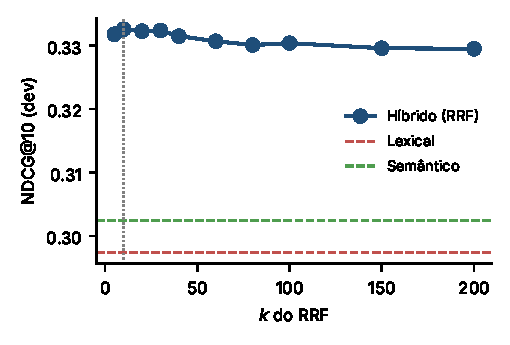
\includegraphics[width=.5\linewidth]{auto/fig_rrf_k.pdf}
\caption{NDCG@10 no \emph{dev} em função de $k$ do RRF; linhas tracejadas: sistemas isolados.}
\label{fig:rrf}
\end{figure}
\begin{table}[t]
\centering
\caption{Parâmetro $k$ do RRF no \textbf{dev}.}
\label{tab:dev_rrf}
\small
\begin{tabular}{rrrrr}
\toprule
$k$ & P@10 & R@10 & MAP@10 & NDCG@10 \\
\midrule
\textit{lexical} & \multicolumn{3}{c}{} & 0,2974 \\
\textit{semântico} & \multicolumn{3}{c}{} & 0,3024 \\
\midrule
5 & 0,2590 & 0,1477 & 0,1080 & 0,3318 \\
10 & 0,2620 & 0,1482 & 0,1082 & 0,3326 \\
20 & 0,2630 & 0,1484 & 0,1079 & 0,3323 \\
30 & 0,2623 & 0,1506 & 0,1080 & 0,3324 \\
40 & 0,2614 & 0,1499 & 0,1077 & 0,3315 \\
60 & 0,2608 & 0,1497 & 0,1077 & 0,3307 \\
80 & 0,2599 & 0,1491 & 0,1075 & 0,3301 \\
100 & 0,2605 & 0,1495 & 0,1075 & 0,3304 \\
150 & 0,2596 & 0,1494 & 0,1074 & 0,3296 \\
200 & 0,2596 & 0,1494 & 0,1073 & 0,3295 \\
\bottomrule
\end{tabular}
\end{table}


\textbf{Cross-encoder.} Em 30 consultas do \emph{dev} (amostra com semente fixa, limitada pelo custo de CPU), o \texttt{ms-marco-MiniLM-L6-v2} elevou o NDCG@10 do híbrido de 0,3642 para 0,3900, enquanto o L12 ficou abaixo do próprio híbrido (0,3581); o L6 foi escolhido (Tabela~\ref{tab:dev_ce}). Veremos na Seção~\ref{sec:rerank} que esse ganho \emph{não} se reproduziu no \emph{test}: 30 consultas são pouco para detectar uma diferença dessa ordem.

\begin{table}[t]
\centering
\caption{Escolha do cross-encoder no \textbf{dev} (amostra de consultas com semente fixa; reordena o Top-50 do híbrido).}
\label{tab:dev_ce}
\small
\begin{tabular}{lrrrrr}
\toprule
Sistema & Consultas & P@10 & R@10 & MAP@10 & NDCG@10 \\
\midrule
hibrido (sem reranking) & 30 & 0,2533 & 0,2004 & 0,1526 & 0,3642 \\
ms-marco-MiniLM-L6-v2 & 30 & 0,2833 & 0,2247 & 0,1601 & 0,3900 \\
ms-marco-MiniLM-L12-v2 & 30 & 0,2700 & 0,2041 & 0,1374 & 0,3581 \\
\bottomrule
\end{tabular}
\end{table}


\textbf{Correção ortográfica.} Em 202 consultas do \emph{dev} com um erro gerado, o NDCG@10 caiu de 0,4489 para 0,1857 e voltou a 0,4428 com $k=\SpK$, Jaccard $\ge \SpJ$ e distância $\le \SpEdit$: o termo exato foi recuperado em 94,6\% dos casos e a recuperação média por consulta foi de 95,0\%. Limiares de Jaccard maiores (0,4 e 0,5) descartam candidatos corretos (acerto de 91,6\% e 85,6\%). Com edição máxima 1 ou 2 o resultado é praticamente igual (0,4428 e 0,4423; Tabela~\ref{tab:dev_spell}); adotamos o critério mais conservador.

\begin{table}[t]
\centering
\caption{Parâmetros da correção ortográfica no \textbf{dev} (202 consultas com um erro gerado; NDCG@10 original = 0,4489, com erro = 0,1857).}
\label{tab:dev_spell}
\footnotesize
\begin{tabular}{rrrrrr}
\toprule
$k$-grama & Jaccard & Edição máx. & Termo corrigido & NDCG@10 corrig. & Recuperação \\
\midrule
2 & 0,2 & 1 & 94,6\% & 0,4428 & 95,0\% \\
2 & 0,2 & 2 & 94,6\% & 0,4423 & 95,0\% \\
2 & 0,3 & 1 & 94,6\% & 0,4428 & 95,0\% \\
2 & 0,3 & 2 & 94,6\% & 0,4423 & 95,0\% \\
2 & 0,4 & 1 & 91,6\% & 0,4361 & 92,3\% \\
2 & 0,4 & 2 & 91,6\% & 0,4359 & 92,4\% \\
2 & 0,5 & 1 & 85,6\% & 0,4255 & 86,9\% \\
2 & 0,5 & 2 & 85,6\% & 0,4252 & 86,8\% \\
3 & 0,2 & 1 & 88,6\% & 0,4333 & 91,6\% \\
3 & 0,2 & 2 & 88,6\% & 0,4304 & 89,8\% \\
3 & 0,3 & 1 & 77,2\% & 0,4135 & 81,6\% \\
3 & 0,3 & 2 & 77,2\% & 0,4122 & 81,4\% \\
3 & 0,4 & 1 & 62,9\% & 0,3768 & 68,1\% \\
3 & 0,4 & 2 & 62,9\% & 0,3816 & 69,4\% \\
3 & 0,5 & 1 & 49,5\% & 0,3478 & 54,0\% \\
3 & 0,5 & 2 & 49,5\% & 0,3478 & 54,0\% \\
\bottomrule
\end{tabular}
\end{table}


\subsection{Lexical $\times$ semântico}
\begin{table}[t]
\centering
\caption{Resultados no \textbf{test} (323 consultas). IC: bootstrap percentil (10.000 reamostragens) sobre as consultas.}
\label{tab:test_main}
\small
\begin{tabular}{lrrrrr}
\toprule
Sistema & P@10 & R@10 & MAP@10 & NDCG@10 & IC 95\% NDCG@10 \\
\midrule
Lexical (BM25) & 0,2406 & 0,1549 & 0,1231 & 0,3303 & [0,296; 0,365] \\
Semântico & 0,2433 & 0,1550 & 0,1108 & 0,3167 & [0,284; 0,352] \\
Híbrido (RRF) & \textbf{0,2607} & \textbf{0,1741} & 0,1353 & 0,3555 & [0,321; 0,392] \\
Híbrido + reranking & 0,2502 & 0,1665 & \textbf{0,1388} & \textbf{0,3557} & [0,321; 0,391] \\
\bottomrule
\end{tabular}
\end{table}

\begin{figure}[t]
\centering
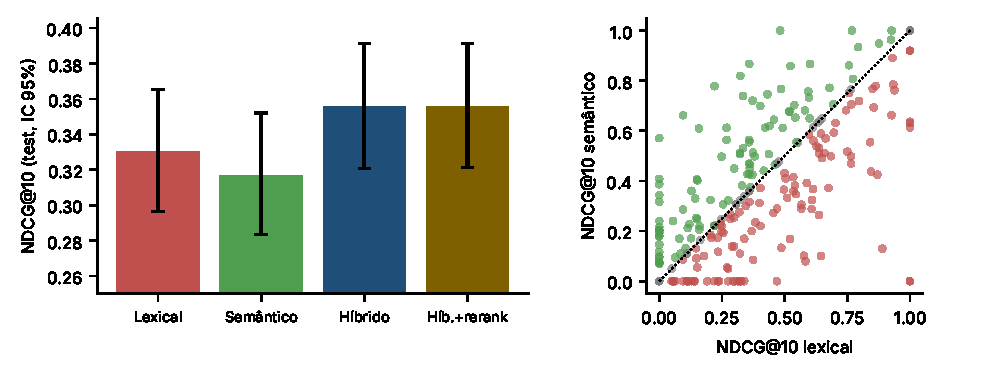
\includegraphics[width=\linewidth]{auto/fig_main.pdf}
\caption{Esquerda: NDCG@10 no \emph{test} por sistema (IC 95\%). Direita: NDCG@10 por consulta, lexical $\times$ semântico (verde: semântico melhor; vermelho: lexical melhor; cinza: empate).}
\label{fig:main}
\end{figure}
\begin{table}[t]
\centering
\caption{Diferenças pareadas por consulta no \textbf{test} (teste de Wilcoxon de postos sinalizados).}
\label{tab:sig}
\small
\begin{tabular}{lrrr}
\toprule
Comparação (A vs.\ B) & $\Delta$ NDCG@10 & A melhor/B melhor/empate & $p$ (Wilcoxon) \\
\midrule
Semântico vs.\ Lexical & -0,0137 & 99/114/110 & 0,312 \\
Híbrido vs.\ Lexical & 0,0252 & 113/77/133 & $<0{,}001$ \\
Híbrido vs.\ Semântico & 0,0388 & 134/69/120 & $<0{,}001$ \\
Híbrido+rerank. vs.\ Híbrido & 0,0002 & 100/99/124 & 0,959 \\
Híbrido+rerank. vs.\ Lexical & 0,0254 & 110/72/141 & $<0{,}001$ \\
Híbrido+rerank. vs.\ Semântico & 0,0391 & 121/95/107 & $<0{,}001$ \\
\bottomrule
\end{tabular}
\end{table}


\textbf{Visão global.} Em média os dois sistemas são equivalentes: NDCG@10 de \NdcgTenLex{} (lexical; o BEIR reporta 0,325 para o BM25 nesta coleção \cite{thakur2021beir}) e \NdcgTenSem{} (semântico), diferença de $-0{,}0137$ sem significância (Wilcoxon, $p=0{,}31$; Tabela~\ref{tab:sig}); P@10 e R@10 são praticamente idênticos e o MAP@10 favorece o lexical (\MapTenLex{} contra \MapTenSem{}). A igualdade média esconde comportamentos muito diferentes por consulta: o semântico vence em \SemWins{} consultas, o lexical em \LexWins{} e há \TieQ{} empates (Figura~\ref{fig:main}), e o Top-10 dos dois sistemas tem Jaccard médio de apenas \OverlapTop. O desencontro de vocabulário é grande: em média \ZeroOverlapPct\% dos documentos relevantes de uma consulta \emph{não contêm nenhum} termo dela (só \AllTermsPct\% contêm todos), e as consultas têm em média \AvgTermsQuery{} termos úteis. \LexNoResult{} consultas do \emph{test} (nomes de alimentos, remédios e lugares, como \emph{eggnog}, \emph{Fosamax}, \emph{okra} e \emph{Yale}) não têm nenhum termo no índice, e o lexical devolve zero resultados; \LexShort{} das 323 consultas têm menos de 100 resultados lexicais. O ganho do semântico cresce com o tamanho da consulta (Spearman entre $\Delta$NDCG e nº de termos: $\rho=\SpearmanNTermsRho$, $p=\SpearmanNTermsP$), mas não se relaciona de forma significativa com a fração de relevantes sem termo da consulta ($\rho=\SpearmanZeroRho$, $p=\SpearmanZeroP$). O tamanho dos documentos recuperados não distingue os sistemas: o Top-10 tem em média \LenTopLex{} tokens no lexical e \LenTopSem{} no semântico, contra \LenCollection{} na coleção e \LenRelevant{} nos relevantes.

\textbf{Os seis casos (Tabelas~\ref{tab:case1}--\ref{tab:case6}).} As três consultas com maior vantagem do semântico e as três com maior vantagem do lexical foram selecionadas automaticamente pela diferença de NDCG@10. Cada análise se apoia nos valores das tabelas e em \texttt{results/\allowbreak analysis/\allowbreak lex\_vs\_sem\_cases.md}.

\begin{table}[!htb]
\centering
\caption{Caso 1 (vantagem do semântico): PLAIN-3085 --- ``The Difficulty of Arriving at a Vitamin D Recommendation''. NDCG@10: lexical 0,000, semântico 0,571. Relevantes: 2; 0 sem nenhum termo da consulta. Colunas: relevância (0--2), score (BM25 | cosseno), posição no outro sistema, $|d|$ = tokens do documento no índice, ter = termos da consulta presentes.}
\label{tab:case1}
\scriptsize
\begin{tabular}{rlrrrrr|lrrrrr}
\toprule
\# & doc & rel & BM25 & r$_s$ & $|d|$ & ter & doc & rel & cos & r$_l$ & $|d|$ & ter \\
\midrule
1 & MED-3632 & 0 & 12,53 & >100 & 153 & 1 & MED-714 & 0 & 0,701 & 7 & 158 & 2 \\
2 & MED-2765 & 0 & 11,41 & 19 & 160 & 2 & MED-4566 & 0 & 0,641 & 59 & 218 & 1 \\
3 & MED-919 & 0 & 11,27 & 5 & 155 & 2 & MED-4573 & 2 & 0,635 & 19 & 135 & 1 \\
4 & MED-4872 & 0 & 11,16 & 14 & 170 & 2 & MED-4570 & 2 & 0,617 & 47 & 146 & 1 \\
5 & MED-4104 & 0 & 10,39 & >100 & 275 & 2 & MED-919 & 0 & 0,611 & 3 & 155 & 2 \\
\bottomrule
\end{tabular}
\end{table}
\begin{table}[!htb]
\centering
\caption{Caso 2 (vantagem do semântico): PLAIN-1537 --- ``low-carb diets''. NDCG@10: lexical 0,095, semântico 0,662. Relevantes: 45; 16 sem nenhum termo da consulta. Colunas: relevância (0--2), score (BM25 | cosseno), posição no outro sistema, $|d|$ = tokens do documento no índice, ter = termos da consulta presentes.}
\label{tab:case2}
\scriptsize
\begin{tabular}{rlrrrrr|lrrrrr}
\toprule
\# & doc & rel & BM25 & r$_s$ & $|d|$ & ter & doc & rel & cos & r$_l$ & $|d|$ & ter \\
\midrule
1 & MED-4880 & 0 & 25,78 & 2 & 178 & 3 & MED-4515 & 1 & 0,662 & 4 & 233 & 2 \\
2 & MED-2943 & 0 & 7,41 & 43 & 252 & 2 & MED-4880 & 0 & 0,609 & 1 & 178 & 3 \\
3 & MED-1714 & 0 & 7,27 & >100 & 248 & 2 & MED-4514 & 1 & 0,596 & 18 & 308 & 2 \\
4 & MED-4515 & 1 & 6,97 & 1 & 233 & 2 & MED-1616 & 1 & 0,587 & 43 & 241 & 2 \\
5 & MED-2458 & 0 & 6,93 & >100 & 216 & 2 & MED-2586 & 1 & 0,558 & >100 & 238 & 2 \\
\bottomrule
\end{tabular}
\end{table}
\begin{table}[!htb]
\centering
\caption{Caso 3 (vantagem do semântico): PLAIN-924 --- ``cocaine''. NDCG@10: lexical 0,220, semântico 0,778. Relevantes: 32; 31 sem nenhum termo da consulta. Colunas: relevância (0--2), score (BM25 | cosseno), posição no outro sistema, $|d|$ = tokens do documento no índice, ter = termos da consulta presentes.}
\label{tab:case3}
\scriptsize
\begin{tabular}{rlrrrrr|lrrrrr}
\toprule
\# & doc & rel & BM25 & r$_s$ & $|d|$ & ter & doc & rel & cos & r$_l$ & $|d|$ & ter \\
\midrule
1 & MED-3044 & 1 & 20,43 & 1 & 217 & 1 & MED-3044 & 1 & 0,467 & 1 & 217 & 1 \\
2 & - & - & - & >100 & - & - & MED-3054 & 1 & 0,384 & >100 & 128 & 0 \\
3 & - & - & - & >100 & - & - & MED-3055 & 1 & 0,339 & >100 & 139 & 0 \\
4 & - & - & - & >100 & - & - & MED-3052 & 1 & 0,335 & >100 & 139 & 0 \\
5 & - & - & - & >100 & - & - & MED-4790 & 0 & 0,313 & >100 & 130 & 0 \\
\bottomrule
\end{tabular}
\end{table}
\begin{table}[!htb]
\centering
\caption{Caso 4 (vantagem do lexical): PLAIN-1473 --- ``kohlrabi''. NDCG@10: lexical 1,000, semântico 0,000. Relevantes: 1; 0 sem nenhum termo da consulta. Colunas: relevância (0--2), score (BM25 | cosseno), posição no outro sistema, $|d|$ = tokens do documento no índice, ter = termos da consulta presentes.}
\label{tab:case4}
\scriptsize
\begin{tabular}{rlrrrrr|lrrrrr}
\toprule
\# & doc & rel & BM25 & r$_s$ & $|d|$ & ter & doc & rel & cos & r$_l$ & $|d|$ & ter \\
\midrule
1 & MED-4455 & 1 & 12,60 & >100 & 118 & 1 & MED-3947 & 0 & 0,220 & >100 & 169 & 0 \\
2 & - & - & - & >100 & - & - & MED-4660 & 0 & 0,217 & >100 & 139 & 0 \\
3 & - & - & - & >100 & - & - & MED-3441 & 0 & 0,216 & >100 & 79 & 0 \\
4 & - & - & - & >100 & - & - & MED-3447 & 0 & 0,213 & >100 & 112 & 0 \\
5 & - & - & - & >100 & - & - & MED-5024 & 0 & 0,212 & >100 & 92 & 0 \\
\bottomrule
\end{tabular}
\end{table}
\begin{table}[!htb]
\centering
\caption{Caso 5 (vantagem do lexical): PLAIN-2081 --- ``shelf life''. NDCG@10: lexical 1,000, semântico 0,000. Relevantes: 1; 0 sem nenhum termo da consulta. Colunas: relevância (0--2), score (BM25 | cosseno), posição no outro sistema, $|d|$ = tokens do documento no índice, ter = termos da consulta presentes.}
\label{tab:case5}
\scriptsize
\begin{tabular}{rlrrrrr|lrrrrr}
\toprule
\# & doc & rel & BM25 & r$_s$ & $|d|$ & ter & doc & rel & cos & r$_l$ & $|d|$ & ter \\
\midrule
1 & MED-4303 & 1 & 17,36 & 15 & 181 & 2 & MED-1378 & 0 & 0,415 & 54 & 135 & 1 \\
2 & MED-1182 & 0 & 12,90 & >100 & 182 & 2 & MED-2422 & 0 & 0,386 & 61 & 143 & 1 \\
3 & MED-2700 & 0 & 12,05 & >100 & 230 & 2 & MED-2510 & 0 & 0,386 & 30 & 121 & 1 \\
4 & MED-2671 & 0 & 10,15 & 35 & 100 & 2 & MED-4715 & 0 & 0,382 & >100 & 232 & 0 \\
5 & MED-2074 & 0 & 8,72 & 86 & 171 & 2 & MED-1433 & 0 & 0,373 & >100 & 121 & 0 \\
\bottomrule
\end{tabular}
\end{table}
\begin{table}[!htb]
\centering
\caption{Caso 6 (vantagem do lexical): PLAIN-1288 --- ``grapes''. NDCG@10: lexical 0,890, semântico 0,130. Relevantes: 196; 181 sem nenhum termo da consulta. Colunas: relevância (0--2), score (BM25 | cosseno), posição no outro sistema, $|d|$ = tokens do documento no índice, ter = termos da consulta presentes.}
\label{tab:case6}
\scriptsize
\begin{tabular}{rlrrrrr|lrrrrr}
\toprule
\# & doc & rel & BM25 & r$_s$ & $|d|$ & ter & doc & rel & cos & r$_l$ & $|d|$ & ter \\
\midrule
1 & MED-2668 & 1 & 11,68 & 15 & 108 & 1 & MED-3200 & 0 & 0,426 & >100 & 142 & 0 \\
2 & MED-2669 & 1 & 11,41 & 13 & 142 & 1 & MED-398 & 0 & 0,425 & >100 & 90 & 0 \\
3 & MED-2083 & 0 & 11,11 & 5 & 182 & 1 & MED-3207 & 0 & 0,425 & >100 & 90 & 0 \\
4 & MED-1538 & 1 & 11,10 & 26 & 183 & 1 & MED-3210 & 0 & 0,424 & >100 & 206 & 0 \\
5 & MED-1533 & 1 & 10,69 & >100 & 183 & 1 & MED-2083 & 0 & 0,414 & 3 & 182 & 1 \\
\bottomrule
\end{tabular}
\end{table}


\textbf{Caso 1 --- \emph{``The Difficulty of Arriving at a Vitamin D Recommendation''} (PLAIN-3085; lexical 0,000 $\times$ semântico 0,571).} Os dois relevantes contêm só um dos quatro termos (\emph{vitamin}); o BM25 recompensa as palavras raras e pouco informativas da consulta: \emph{arriv} (idf 6,18) e \emph{difficulti} (5,08) pesam mais que \emph{vitamin} (2,79), e o Top-5 lexical traz, por exemplo, o MED-3632, sobre um aumento de mortalidade ``após a chegada'' de algo, sem relação com vitamina D. O primeiro relevante está na posição 19 no lexical e nas posições 3 e 4 no semântico (cossenos 0,635 e 0,617): o embedding capta o tema (\emph{recomendação sobre vitamina D}) em vez de somar palavras raras. Evidência de \textbf{peso excessivo de termos raros e de paráfrase}.

\textbf{Caso 2 --- \emph{``low-carb diets''} (PLAIN-1537; 0,095 $\times$ 0,662).} \emph{carb} aparece em um único documento (df $=1$, idf 7,79) porque os textos escrevem \emph{carbohydrate}: abreviação $\times$ forma plena (\textbf{variação de vocabulário e sinonímia}). Esse documento, não relevante, domina o ranking lexical (score 25,8 contra 7,4 do segundo), e os demais documentos lexicais casam só com \emph{low} e \emph{diet} (dietas hipocalóricas, hipoproteicas). Dos 45 relevantes, 16 não têm nenhum termo da consulta; o semântico coloca 4 relevantes no Top-5 e 6 no Top-10 (lexical: 1 e 1).

\textbf{Caso 3 --- \emph{``cocaine''} (PLAIN-924; 0,220 $\times$ 0,778).} Só um documento da coleção contém \emph{cocain}; o lexical devolve apenas esse resultado (relevante, posição 1), de modo que o recall fica limitado a 1/32: 31 dos 32 relevantes não contêm o termo. O semântico mantém esse documento no topo e acrescenta textos sobre vício em comida e circuitos de recompensa (MED-3054, MED-3055, MED-3052, todos relevantes) que nunca citam cocaína: a \textbf{relevância é temática e indireta}. Há 18 relevantes no Top-100 semântico contra 1 no lexical.

\textbf{Caso 4 --- \emph{``kohlrabi''} (PLAIN-1473; 1,000 $\times$ 0,000).} O único relevante (MED-4455) contém o termo raro (df $=1$, idf 7,79), logo o BM25 o coloca em 1º. O tokenizador do bi-encoder fragmenta \emph{kohlrabi} em \texttt{ko\,\#\#hl\,\#\#ra\,\#\#bi}, peças sem relação com a hortaliça; os documentos devolvidos (algas, hibisco) têm cosseno máximo de 0,22 e o relevante fica fora do Top-100. Evidência a favor da \textbf{correspondência exata de termos técnicos e nomes raros}.

\textbf{Caso 5 --- \emph{``shelf life''} (PLAIN-2081; 1,000 $\times$ 0,000).} O relevante (MED-4303, ``shelf-life evaluation of selected culinary oils'') contém os dois termos e o BM25 o ranqueia em 1º (\emph{shelf}: idf 6,18). O semântico interpreta \emph{life} como tempo de vida: o Top-5 é sobre longevidade, restrição calórica e envelhecimento (por exemplo ``Longevity and diet. Myth or pragmatism?''), e o relevante só aparece na posição 15. É um caso de \textbf{ambiguidade} (\emph{shelf life} $\ne$ \emph{life}).

\textbf{Caso 6 --- \emph{``grapes''} (PLAIN-1288; 0,890 $\times$ 0,130).} Dos 196 relevantes, apenas 15 contêm \emph{grape}, mas são eles que o lexical coloca no topo (9 relevantes no Top-10). O semântico traz no Top-5 quatro documentos sobre \emph{grapefruit} (nenhum relevante), cujo termo é segmentado em \texttt{grape\,\#\#fr\,\#\#uit}, ou seja, compartilha a peça \emph{grape} e o domínio ``fruta cítrica/fruta''; o primeiro relevante está na posição 9. Em consulta de uma só palavra, sem contexto, a \textbf{vizinhança lexical e semântica} do embedding produz ruído que a correspondência exata evita. (Os documentos MED-398 e MED-3207 têm o mesmo título e o mesmo cosseno, ou seja, são duplicatas na coleção.)

\subsection{Tolerância a erros ortográficos}
\begin{table}[t]
\centering
\caption{Experimento de tolerância a erros (sistema lexical, \textbf{test}). Recup. = (corrigida $-$ erro)/(original $-$ erro).}
\label{tab:typo}
\scriptsize
\begin{tabular}{llllllrrr}
\toprule
Consulta & Tipo de erro & Original & Com erro & Corrigido & NDCG orig. & NDCG erro & NDCG corr. & Recup. \\
\midrule
PLAIN-344 & substituição & \texttt{dioxins} & \texttt{diofins} & \texttt{dioxins} & 0,417 & 0,000 & 0,417 & 100\% \\
PLAIN-1527 & inserção & \texttt{liver} & \texttt{livwer} & \texttt{liver} & 0,768 & 0,069 & 0,768 & 100\% \\
PLAIN-1172 & remoção & \texttt{fenugreek} & \texttt{feugreek} & \texttt{fenugreek} & 0,220 & 0,000 & 0,220 & 100\% \\
PLAIN-711 & troca & \texttt{clots} & \texttt{colts} & \texttt{costs} & 0,359 & 0,000 & 0,000 & 0\% \\
PLAIN-2124 & substituição & \texttt{spearmint} & \texttt{skearmint} & \texttt{spearmint} & 0,359 & 0,000 & 0,359 & 100\% \\
PLAIN-2040 & inserção & \texttt{salmon} & \texttt{saglmon} & \texttt{salmon} & 0,751 & 0,000 & 0,751 & 100\% \\
PLAIN-1983 & remoção & \texttt{rapamycin} & \texttt{raamycin} & \texttt{rapamycin} & 1,000 & 0,000 & 1,000 & 100\% \\
PLAIN-1601 & troca & \texttt{memory} & \texttt{mmeory} & \texttt{memory} & 0,581 & 0,000 & 0,581 & 100\% \\
PLAIN-701 & substituição & \texttt{raspberries} & \texttt{raspberrieh} & \texttt{raspberries} & 0,510 & 0,084 & 0,510 & 100\% \\
PLAIN-1473 & inserção & \texttt{kohlrabi} & \texttt{kohlrrabi} & \texttt{kohlrabi} & 1,000 & 0,000 & 1,000 & 100\% \\
\bottomrule
\end{tabular}
\end{table}

Das \TypoEligible{} consultas elegíveis do \emph{test} (NDCG@10 original $>0$), 10 foram sorteadas, com os quatro tipos de erro atribuídos em rodízio (3 substituições, 3 inserções, 2 remoções, 2 trocas). O NDCG@10 médio do sistema lexical foi de \TypoOrig{} (original) para \TypoErr{} (com erro) e \TypoCorr{} (corrigida): a correção recuperou \TypoRecAgg\% da queda (agregado) e \TypoRecMean\% em média por consulta; em todas as \TypoNDrop{} consultas o erro reduziu o NDCG@10 (nenhuma ficou sem queda), e \TypoNExact{} correções devolveram exatamente o termo original (Tabela~\ref{tab:typo}). A queda é quase total porque várias consultas têm um ou dois termos (\emph{fenugreek}, \emph{salmon}, \emph{memory}\ldots): o erro cria um termo inexistente, com zero \emph{postings}, e nada é recuperado.

\textbf{O caso que falhou} (PLAIN-711, \emph{blood clots} $\rightarrow$ \emph{blood colts}, troca de ordem): todos os candidatos a distância 1 são ``vizinhos'' do erro: \emph{costs} (Jaccard 0,50; frequência 87), \emph{colas}, \emph{coats}, \emph{colds} (0,50) e, por último, \emph{clots} (0,33; frequência 1). A troca de duas letras adjacentes custa 1 na distância de edição, mas altera três bigramas (\texttt{ol}, \texttt{lt}, \texttt{ts}$\rightarrow$\texttt{lo}, \texttt{ot}, \texttt{ts}), e o desempate por Jaccard e depois por frequência escolhe \emph{costs}: NDCG@10 permanece 0 (recuperação 0\%). Uma correção sensível ao contexto (\emph{blood} coocorre com \emph{clots}) ou um modelo de canal ruidoso resolveria o caso; não foi implementada. A amostra de 10 consultas é pequena (a de 202 consultas do \emph{dev} dá recuperação média de 95,0\%).

\textbf{Sistema semântico (opcional).} Com as mesmas consultas, o NDCG@10 do bi-encoder cai de 0,5173 para 0,1240 com o erro e volta a 0,4747 com a consulta corrigida (recuperação média de 87,5\% nas 8 consultas em que o erro reduziu o desempenho; nas outras 2 não houve queda). Os embeddings, portanto, também são frágeis a erros de digitação: o erro altera as peças do tokenizador (\emph{fenugreek}: \texttt{fen\,\#\#ug\,\#\#ree\,\#\#k}; \emph{feugreek}: \texttt{fe\,\#\#ug\,\#\#ree\,\#\#k}), o que muda o vetor da consulta. A correção, aplicada antes da codificação, serve aos dois sistemas.

\subsection{Busca híbrida}
O RRF com $k=\RrfK$ eleva o NDCG@10 do \emph{test} para \NdcgTenHyb{}: $+0{,}0252$ sobre o lexical ($p=7{,}3\times10^{-5}$) e $+0{,}0388$ sobre o semântico ($p=3{,}5\times10^{-7}$); P@10 passa a \PTenHyb{} e R@10 a \RTenHyb{} (Tabela~\ref{tab:test_main}). O híbrido é melhor que \emph{ambos} os sistemas em \HybBeatBoth{} consultas e pior que ambos em apenas \HybLoseBoth{}; nas demais \HybBetween{} fica igual ou entre os dois. A explicação está na complementaridade medida: o Recall@100 é \RecLexHundred{} no lexical, \RecSemHundred{} no semântico e \RecUnionHundred{} na união; dos relevantes encontrados por algum sistema, \OnlyLexPct\% só pelo lexical, \OnlySemPct\% só pelo semântico e \BothPct\% por ambos. O RRF premia documentos que aparecem nos dois rankings sem comparar escores de escalas diferentes (BM25 e cosseno). Um efeito colateral são os empates de RRF (um documento em 1º só no lexical e outro em 1º só no semântico têm o mesmo escore), resolvidos aqui pelo identificador, o que aparece no caso \emph{kohlrabi} adiante.

\subsection{Reranking}\label{sec:rerank}
\begin{figure}[t]
\centering
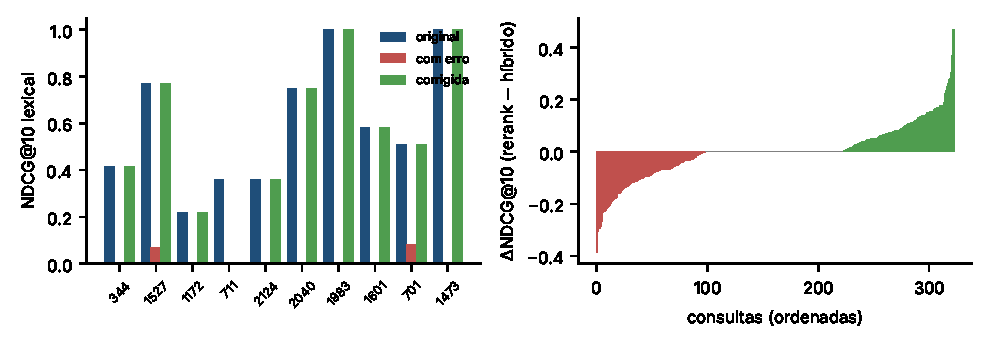
\includegraphics[width=\linewidth]{auto/fig_typo_rerank.pdf}
\caption{Esquerda: NDCG@10 lexical nas 10 consultas do experimento de erros. Direita: $\Delta$NDCG@10 por consulta do reranking (híbrido+reranking $-$ híbrido), ordenado.}
\label{fig:typo_rerank}
\end{figure}
\textbf{Resultado global.} O reranking com o cross-encoder \emph{não} melhorou o NDCG@10 do \emph{test}: \NdcgTenHyb{} (híbrido) contra \NdcgTenRr{} (híbrido+reranking), $\Delta=+0{,}0002$ ($p=0{,}96$). P@10 e R@10 \emph{caíram} (de \PTenHyb{} para \PTenRr{} e de \RTenHyb{} para \RTenRr{}) e o MAP@10 subiu levemente (\MapTenHyb{} $\rightarrow$ \MapTenRr{}). Por consulta, \RrBetter{} melhoraram, \RrWorse{} pioraram e \RrSame{} não mudaram (Figura~\ref{fig:typo_rerank}, painel direito). Havia muito a ganhar: o Top-50 híbrido contém em média \RecFiftyHyb{} dos relevantes e um reordenador perfeito dele alcançaria NDCG@10 de \OracleNdcg{}; o cross-encoder promoveu \RelPromoted{} relevantes das posições 11--50 para o Top-10, mas rebaixou \RelDemoted{} relevantes para fora dele (saldo negativo, coerente com a queda de P@10). O Top-10 pós-reranking tem documentos mais longos (\LenTopRer{} tokens contra \LenTopHyb{} no híbrido e \LenCollection{} na coleção). O ganho de +0,026 visto no \emph{dev} provavelmente refletia a variância de uma amostra de apenas 30 consultas. O resultado do \emph{test} é compatível com o que o BEIR reporta para BM25 + cross-encoder MiniLM no NFCorpus (NDCG@10 de 0,350 \cite{thakur2021beir}): o híbrido já chega a esse patamar sem o reranker. (Hipóteses não testadas aqui: o cross-encoder foi treinado no MS MARCO, com consultas e trechos de web, enquanto no NFCorpus a relevância é derivada de citações e muitas vezes é indireta.)

\begin{table}[!htb]
\centering
\caption{Reranking, caso 1 (maior ganho 1): PLAIN-1320 --- ``Harvard Physicians' Study II''. NDCG@10: híbrido 0,091 $\rightarrow$ 0,562. Documentos do Top-10 (antes ou depois) com maior deslocamento, ordenados pela posição final. $\Delta$ = posição híbrida $-$ posição final.}
\label{tab:rr1}
\scriptsize
\begin{tabular}{rrrlrrrrrr}
\toprule
rank CE & rank híb. & $\Delta$ & doc & rel & score CE & r$_{lex}$ & r$_{sem}$ & $|d|$ & ter \\
\midrule
5 & 19 & +14 & MED-4398 & 0 & -4,21 & 5 & >100 & 157 & 3 \\
6 & 22 & +16 & MED-2761 & 1 & -5,36 & 11 & 84 & 205 & 3 \\
7 & 26 & +19 & MED-3932 & 0 & -6,24 & 10 & >100 & 188 & 3 \\
8 & 46 & +38 & MED-5124 & 0 & -7,14 & 24 & >100 & 205 & 2 \\
10 & 39 & +29 & MED-1622 & 0 & -7,52 & 21 & >100 & 184 & 3 \\
16 & 1 & -15 & MED-1053 & 0 & -8,55 & 6 & 4 & 144 & 2 \\
17 & 3 & -14 & MED-1097 & 0 & -8,66 & 14 & 3 & 86 & 1 \\
28 & 2 & -26 & MED-2112 & 0 & -9,78 & 17 & 1 & 64 & 2 \\
\bottomrule
\end{tabular}
\end{table}
\begin{table}[!htb]
\centering
\caption{Reranking, caso 2 (maior ganho 2): PLAIN-1473 --- ``kohlrabi''. NDCG@10: híbrido 0,631 $\rightarrow$ 1,000. Documentos do Top-10 (antes ou depois) com maior deslocamento, ordenados pela posição final. $\Delta$ = posição híbrida $-$ posição final.}
\label{tab:rr2}
\scriptsize
\begin{tabular}{rrrlrrrrrr}
\toprule
rank CE & rank híb. & $\Delta$ & doc & rel & score CE & r$_{lex}$ & r$_{sem}$ & $|d|$ & ter \\
\midrule
4 & 48 & +44 & MED-1686 & 0 & -6,73 & >100 & 47 & 106 & 0 \\
7 & 45 & +38 & MED-2135 & 0 & -8,07 & >100 & 44 & 197 & 0 \\
9 & 36 & +27 & MED-712 & 0 & -8,42 & >100 & 35 & 186 & 0 \\
40 & 10 & -30 & MED-744 & 0 & -10,23 & >100 & 9 & 124 & 0 \\
41 & 6 & -35 & MED-5024 & 0 & -10,24 & >100 & 5 & 92 & 0 \\
43 & 7 & -36 & MED-4385 & 0 & -10,38 & >100 & 6 & 87 & 0 \\
44 & 3 & -41 & MED-4660 & 0 & -10,43 & >100 & 2 & 139 & 0 \\
47 & 4 & -43 & MED-3441 & 0 & -10,89 & >100 & 3 & 79 & 0 \\
\bottomrule
\end{tabular}
\end{table}
\begin{table}[!htb]
\centering
\caption{Reranking, caso 3 (pouca/nenhuma alteração): PLAIN-1557 --- ``magnesium''. NDCG@10: híbrido 0,315 $\rightarrow$ 0,315. Documentos do Top-10 (antes ou depois) com maior deslocamento, ordenados pela posição final. $\Delta$ = posição híbrida $-$ posição final.}
\label{tab:rr3}
\scriptsize
\begin{tabular}{rrrlrrrrrr}
\toprule
rank CE & rank híb. & $\Delta$ & doc & rel & score CE & r$_{lex}$ & r$_{sem}$ & $|d|$ & ter \\
\midrule
2 & 3 & +1 & MED-3918 & 1 & -0,53 & 3 & 3 & 98 & 1 \\
3 & 2 & -1 & MED-4315 & 1 & -1,36 & 4 & 2 & 82 & 1 \\
5 & 11 & +6 & MED-5005 & 0 & -2,69 & 7 & >100 & 259 & 1 \\
7 & 27 & +20 & MED-3497 & 0 & -3,80 & 16 & >100 & 180 & 1 \\
8 & 41 & +33 & MED-2249 & 0 & -3,90 & 23 & >100 & 237 & 1 \\
15 & 7 & -8 & MED-1844 & 0 & -5,36 & >100 & 5 & 167 & 0 \\
30 & 5 & -25 & MED-1110 & 0 & -7,06 & >100 & 4 & 139 & 0 \\
34 & 8 & -26 & MED-1843 & 0 & -7,97 & >100 & 6 & 143 & 0 \\
\bottomrule
\end{tabular}
\end{table}
\begin{table}[!htb]
\centering
\caption{Reranking, caso 4 (piora): PLAIN-1679 --- ``myelopathy''. NDCG@10: híbrido 0,387 $\rightarrow$ 0,000. Documentos do Top-10 (antes ou depois) com maior deslocamento, ordenados pela posição final. $\Delta$ = posição híbrida $-$ posição final.}
\label{tab:rr4}
\scriptsize
\begin{tabular}{rrrlrrrrrr}
\toprule
rank CE & rank híb. & $\Delta$ & doc & rel & score CE & r$_{lex}$ & r$_{sem}$ & $|d|$ & ter \\
\midrule
1 & 32 & +31 & MED-1105 & 0 & 0,19 & >100 & 32 & 83 & 0 \\
2 & 24 & +22 & MED-1104 & 0 & -0,93 & >100 & 24 & 62 & 0 \\
6 & 19 & +13 & MED-1111 & 0 & -2,88 & >100 & 19 & 195 & 0 \\
9 & 2 & -7 & MED-1113 & 0 & -4,11 & >100 & 2 & 185 & 0 \\
10 & 39 & +29 & MED-4312 & 0 & -5,22 & >100 & 39 & 77 & 0 \\
15 & 7 & -8 & MED-3302 & 0 & -7,58 & >100 & 7 & 111 & 0 \\
37 & 1 & -36 & MED-5133 & 0 & -9,98 & >100 & 1 & 89 & 0 \\
40 & 5 & -35 & MED-5142 & 1 & -10,20 & >100 & 5 & 129 & 0 \\
\bottomrule
\end{tabular}
\end{table}


\textbf{Maior ganho 1 --- PLAIN-1320, \emph{``Harvard Physicians' Study II''} (0,091 $\rightarrow$ 0,562; relevantes no Top-10: 1 $\rightarrow$ 3).} O cross-encoder subiu os três relevantes sobre o \emph{Physicians' Health Study} (MED-2760: posição 9 $\rightarrow$ 1, escore 0,755; MED-2758: 12 $\rightarrow$ 3; MED-2761: 22 $\rightarrow$ 6). O semântico havia posto esses documentos nas posições 74, 38 e 84, favorecendo textos sobre médicos em geral (posições 1 a 4: \emph{``How evidence-based medicine biases physicians against nutrition''}, \emph{``Physician disclosure\ldots''}), enquanto o lexical os tinha em 2, 4 e 11. Lendo consulta e documento juntos, o reranker casou o nome próprio ``Physicians' Health Study'' do título; os quatro documentos que o semântico havia posto em 1º a 4º lugar foram para as posições 9, 16, 17 e 28. (O MED-4929, também do \emph{Physicians' Health Study II}, está em 2º e é não relevante no qrels, um sinal de julgamentos incompletos.)

\textbf{Maior ganho 2 --- PLAIN-1473, \emph{``kohlrabi''} (0,631 $\rightarrow$ 1,000).} O único relevante já estava em 2º no híbrido: o 1º era o MED-3947 (hibisco), com o mesmo escore RRF $1/(10+1)$ do relevante (1º só no semântico $\times$ 1º só no lexical); o desempate por identificador favoreceu o irrelevante. O cross-encoder deu +1,22 ao MED-4455 (que contém o termo) contra $-4{,}31$ ao seguinte. O ``ganho'' é a correção de um empate do RRF, e o semântico não tinha informação sobre \emph{kohlrabi} (Caso 4).

\textbf{Pouca ou nenhuma alteração --- PLAIN-1557, \emph{``magnesium''} ($\Delta=0$).} Os três relevantes continuam no Top-10 (posições híbridas 3, 2 e 9; finais 2, 3 e 9): só trocaram de lugar os dois primeiros, ambos com grau 1, o que não altera o NDCG. Cinco posições do Top-10 mudam, mas por documentos não relevantes que entram vindo de mais fundo (MED-3497: 27 $\rightarrow$ 7). Todos os documentos do topo já continham o termo \emph{magnesium}, de modo que o reranker não tinha sinal novo para separá-los.

\textbf{Piora --- PLAIN-1679, \emph{``myelopathy''} (0,387 $\rightarrow$ 0,000).} A palavra não existe no índice (df $=0$): o híbrido é só o ranking semântico, que põe o único relevante (MED-5142, degeneração combinada subaguda da medula espinhal) na posição 5. O cross-encoder o rebaixa para a 40ª (escore $-10{,}2$) e coloca no topo textos sobre \emph{mieloma múltiplo} (por exemplo o MED-1105, escore 0,193): \emph{myelopathy} e \emph{myeloma} compartilham as peças \texttt{my\,\#\#elo} no tokenizador, e o documento relevante nunca usa a palavra da consulta. O modelo, treinado em passagens de web, não conhece a relação clínica e se apoia na forma da palavra.

\subsection{Tempos}
\begin{table}[t]
\centering
\caption{Tempos medidos (CPU: Intel(R) Xeon(R) Processor @ 2.10GHz, 1 núcleo(s), sem GPU).}
\label{tab:times}
\small
\begin{tabular}{lrl}
\toprule
Etapa & Tempo & Frequência \\
\midrule
Índice invertido (pré-processamento + estruturas) & 1,23 s & uma vez \\
Embeddings dos documentos (3.633) & 219 s & uma vez \\
Consulta lexical (pré-proc. + BM25 + Top-100) & 0,25 ms & por consulta \\
Consulta semântica (codificação + busca exaustiva) & 3,5 ms & por consulta \\
Fusão RRF (100 + 100 documentos) & 0,102 ms & por consulta \\
Reranking (cross-encoder, 50 pares) & 12,3 s & por consulta \\
\bottomrule
\end{tabular}
\end{table}

Medidos em CPU de um único núcleo (Tabela~\ref{tab:times}): o índice invertido é construído em \IdxTotal{} s e responde em \LexMs{} ms por consulta; os embeddings dos documentos levam \EncDocSeconds{} s e a consulta semântica, \EncQueryMs{} ms; a fusão RRF custa \RrfMs{} ms. O reranking de 50 pares leva \CEMsQuery{} s por consulta (\CESecPair{} s por par, com média de \CEPairTokens{} tokens por par), muito mais que todo o restante junto, e foi implementado com NumPy puro em CPU; em GPU o custo seria muito menor, mas a proporção entre as etapas deve se manter. Sem reranking, a consulta híbrida completa leva cerca de 4 ms.

\subsection{RAG}
\textbf{Recuperação (Top-5 pós-reranking enviado à LLM).} Pelo menos um documento relevante chegou ao contexto em 9 das 10 consultas (Hit@5 $=$ \RagHit), com Precision@5 médio de \RagPrec{} e Recall@5 médio de \RagRecall{} (Tabela~\ref{tab:rag_ret}). O Recall@5 baixo é esperado: as consultas têm em média 43,6 relevantes, então 5 documentos cobrem no máximo cerca de 11,5\%. O caso extremo é PLAIN-153 (\emph{How Should I Take Probiotics?}), em que os 5 documentos são relevantes; a exceção é PLAIN-2850 (\emph{More Antibiotics In White Meat or Dark Meat?}), sem nenhum relevante no contexto.
\begin{table}[t]
\centering
\caption{RAG: recuperação nos Top-5 enviados à LLM (após reranking). ``Graus no Top-5'' = relevância de cada documento do contexto (0 = não relevante/não julgado).}
\label{tab:rag_ret}
\scriptsize
\begin{tabular}{llrlrrr}
\toprule
Consulta & Pergunta & Rel. total & Graus no Top-5 & R@5 & P@5 & Hit@5 \\
\midrule
PLAIN-68 & What is Actually in Chicken Nuggets? & 55 & 2 0 0 0 0 & 0,018 & 0,20 & 1 \\
PLAIN-2450 & Are Organic Foods Safer? & 38 & 0 2 0 0 2 & 0,053 & 0,40 & 1 \\
PLAIN-153 & How Should I Take Probiotics? & 47 & 2 1 1 1 1 & 0,106 & 1,00 & 1 \\
PLAIN-2850 & More Antibiotics In White Meat or Dark Meat? & 9 & 0 0 0 0 0 & 0,000 & 0,00 & 0 \\
PLAIN-2750 & Preventing the Common Cold with Probiotics? & 59 & 2 1 2 1 0 & 0,068 & 0,80 & 1 \\
PLAIN-270 & Is Caffeinated Tea Really Dehydrating? & 52 & 1 0 0 0 1 & 0,038 & 0,40 & 1 \\
PLAIN-2470 & Is Milk Good for Our Bones? & 73 & 2 2 2 0 0 & 0,041 & 0,60 & 1 \\
PLAIN-2430 & Preventing Brain Loss with B Vitamins? & 46 & 2 2 0 2 0 & 0,065 & 0,60 & 1 \\
PLAIN-238 & How Chemically Contaminated Are We? & 54 & 0 1 0 0 0 & 0,018 & 0,20 & 1 \\
PLAIN-3342 & Is Coconut Milk Good For You? & 3 & 2 0 0 0 2 & 0,667 & 0,40 & 1 \\
\textbf{Média} &  &  &  & 0,107 & 0,46 & 0,9 \\
\bottomrule
\end{tabular}
\end{table}


\textbf{Geração: configuração e verificações objetivas.} A LLM é a descrita na Metodologia; as respostas têm em média \RagWordsA{} palavras na condição A e \RagWordsB{} na B. As respostas B citam \RagCited{} documentos no total, \textbf{todos presentes no contexto enviado} (\RagCitedValid{} de \RagCited{}, nenhum identificador inventado); \RagCitedRel{} das citações apontam para documentos relevantes no qrels, porque várias respostas citam documentos irrelevantes justamente para dizer que eles não tratam da pergunta (\RagCtxRel{} dos \RagCtxN{} documentos do contexto são relevantes). As respostas A não têm fontes (0 identificadores), como previsto. Estas verificações automáticas \emph{não substituem} a avaliação humana.

\textbf{Avaliação humana (Tabela~\ref{tab:rag_grades}).} \todo{A preencher pelos integrantes: avaliar a planilha cega (results/\allowbreak rag\_annotation\_sheet.csv) com o script 07 e atualizar esta tabela e o texto abaixo. Discutir as médias A $\times$ B por critério, a concordância entre avaliadores e a ausência de fontes na condição A (rastreabilidade N/A).}
\begin{table}[t]
\centering
\caption{RAG: médias das notas da avaliação humana (0--2) por condição. \textbf{PENDENTE}: preencher após a avaliação humana (script 07).}
\label{tab:rag_grades}
\small
\begin{tabular}{lrrrr}
\toprule
Condição & Fidelidade & Completude & Utilidade & Rastreabilidade \\
\midrule
A (sem RAG) & \textit{a preencher} & \textit{a preencher} & \textit{a preencher} & N/A \\
B (com RAG) & \textit{a preencher} & \textit{a preencher} & \textit{a preencher} & \textit{a preencher} \\
\bottomrule
\end{tabular}
\end{table}


\subsection{Análise de falhas ponta a ponta}
\todo{Escolher, depois das notas, três consultas: (1) o RAG melhorou claramente a resposta; (2) pouca diferença; (3) o RAG não ajudou ou prejudicou. Para a (3), localizar o estágio do problema (lexical, semântico, fusão, reranking, seleção de contexto ou geração) com results/\allowbreak analysis/\allowbreak rag\_failure\_traces.md.}
\textbf{Evidência já disponível para um candidato à categoria (3): PLAIN-2850.} Existem 9 relevantes no qrels e nenhum chegou ao Top-10 em nenhuma etapa: em cada sistema só 2 deles estão no Top-100 e o primeiro relevante aparece na posição 77 (lexical), 14 (semântico), 38 (híbrido) e 16 (reranking). A informação necessária, portanto, nunca chegou ao contexto: o problema está na \textbf{recuperação} (os dois recuperadores falham e a fusão e o reranking não os salvam), não na geração. A resposta B declara que o contexto não tem evidência suficiente, o que é fiel ao contexto, mas pouco útil; os documentos recuperados tratam de resistência bacteriana em carnes de varejo, bacteriófagos e consumo de carne e doenças, sem comparar carne branca e escura. Confirme a classificação com as notas.

\subsection{Limitações}
(i) A escolha do cross-encoder usou só 30 consultas do \emph{dev} e não se confirmou no \emph{test}. (ii) O experimento de erros usa 10 consultas e um erro por consulta; o \emph{dev} (202 consultas) corrobora o resultado. (iii) Os qrels do NFCorpus são incompletos e derivados de citações (por exemplo, o MED-4929 é tematicamente adequado ao caso PLAIN-1320, mas não é relevante), o que subestima todos os sistemas. (iv) Cada sistema foi executado uma vez, sem repetições. (v) A LLM do RAG foi usada por interface de chat, sem controle de temperatura ou semente. (vi) Tempos medidos em uma CPU de um núcleo.

\section{Considerações Finais}
\textbf{(1) Lexical e semântico são equivalentes em média e complementares por consulta.} BM25 e bi-encoder têm NDCG@10 de \NdcgTenLex{} e \NdcgTenSem{} no \emph{test} (diferença sem significância), mas ganham em consultas diferentes: o lexical vence quando há termo raro ou nome próprio (\emph{kohlrabi}, \emph{shelf life}, \emph{grapes}), e o semântico quando há sinonímia, abreviação, relevância indireta ou palavras raras sem valor temático (\emph{low-carb}, \emph{cocaine}, \emph{vitamin D recommendation}). Os Top-10 se sobrepõem pouco (Jaccard \OverlapTop).
\textbf{(2) O RRF é a melhoria mais barata e consistente:} $+0{,}025$ de NDCG@10 sobre o lexical e $+0{,}039$ sobre o semântico, com sensibilidade pequena a $k$ e custo de décimos de milissegundo.
\textbf{(3) A correção ortográfica funciona, mas é frágil em empates:} recuperou \TypoRecAgg\% da queda de NDCG@10 nas 10 consultas do \emph{test} (95\% no \emph{dev}); a única falha foi uma troca de letras cujo candidato correto perdeu no desempate por Jaccard e frequência. Os embeddings também sofrem com erros de digitação.
\textbf{(4) O reranking com o cross-encoder MS MARCO MiniLM não compensou o custo neste experimento:} NDCG@10 de \NdcgTenHyb{} para \NdcgTenRr{} ($p=0{,}96$), P@10 menor, e \CEMsQuery{} s por consulta em CPU. Há margem (oráculo de \OracleNdcg{} no Top-50), mas o modelo a aproveita mal; vale testar um cross-encoder treinado no domínio biomédico e mais consultas do \emph{dev} na escolha.
\textbf{(5) RAG:} a recuperação entregou ao menos um relevante ao contexto em 9 de 10 consultas, e a única exceção (PLAIN-2850) é uma falha de recuperação, não de geração. \todo{Concluir, após a avaliação humana, o efeito do RAG na fidelidade, completude, utilidade e rastreabilidade.}
\textbf{Trabalhos futuros:} correção sensível ao contexto, expansão de consultas para termos fora do vocabulário (nomes de remédios, alimentos e lugares), fusão ponderada ou aprendida, reranker específico de domínio e avaliação do RAG com mais consultas e mais de uma LLM.

\section{Uso de ferramentas de IA}
\textbf{IA como componente do experimento} (documentada na Metodologia): o bi-encoder \texttt{\EncName}, o cross-encoder \texttt{\CEName} e a LLM do RAG. \textbf{IA como apoio ao desenvolvimento:} usamos o assistente Claude (Anthropic) para escrever e depurar o código do projeto (índice invertido, BM25, correção ortográfica, métricas, scripts e testes), planejar e executar os experimentos, gerar tabelas e figuras, rascunhar o texto deste relatório e as análises por consulta a partir das evidências numéricas produzidas pelo código, e redigir as respostas das duas condições do experimento de RAG. Os integrantes revisaram o código, os resultados e o texto e são responsáveis por compreendê-los e defendê-los. A avaliação humana do RAG (notas de 0 a 2) cabe aos integrantes e não foi delegada à IA.
% CONFIRMAR antes de entregar: ajuste esta seção ao uso real de ferramentas de IA pelo grupo.

\bibliography{refs}
\end{document}
